
%%%%%%%%%%%%%%%%%%%%%%% file typeinst.tex %%%%%%%%%%%%%%%%%%%%%%%%%
%
% This is the LaTeX source for the instructions to authors using
% the LaTeX document class 'llncs.cls' for contributions to
% the Lecture Notes in Computer Sciences series.
% http://www.springer.com/lncs       Springer Heidelberg 2006/05/04
%
% It may be used as a template for your own input - copy it
% to a new file with a new name and use it as the basis
% for your article.
%
% NB: the document class 'llncs' has its own and detailed documentation, see
% ftp://ftp.springer.de/data/pubftp/pub/tex/latex/llncs/latex2e/llncsdoc.pdf
%
%%%%%%%%%%%%%%%%%%%%%%%%%%%%%%%%%%%%%%%%%%%%%%%%%%%%%%%%%%%%%%%%%%%

%\modelname, \modelname

%\documentclass[runningheads,a4paper]{llncs}
\documentclass[a4paper]{llncs}

\usepackage{tikz}
\usetikzlibrary{positioning,fit}

\usepackage{amssymb}
\setcounter{tocdepth}{3}
\usepackage{graphicx}
%%%%TODO: REMOVE THE TERM metacompleteness
%% MY COOL PACKAGES
\usepackage[utf8]{inputenc}
\usepackage[T1]{fontenc}
%\usepackage{times}
\usepackage{tgtermes}
%\usepackage{bera}
\usepackage[scaled=0.93]{beramono}
\usepackage[normalem]{ulem}
\usepackage{cite}
\usepackage{float}
\usepackage{wrapfig}
\usepackage{scalefnt}
\usepackage{setspace}
%
%\usepackage{listings}
%\lstset{basicstyle=\ttfamily\small, 
%%  numbers=left, numberstyle=\tiny, stepnumber=1, numbersep=5pt,
%  language=java, mathescape=true, escapechar=\!,
%  emph={object}, emphstyle=\textbf,
%  showstringspaces=false
%}
%%%%

\usepackage{hyperref}
\usepackage{xcolor}
\definecolor{entityColor}{RGB}{0,100,200}
\definecolor{attributeColor}{RGB}{0,100,50}
\definecolor{relationColor}{RGB}{160,0,30}
\usepackage{listings}
\lstdefinestyle{reqT}{
  %belowcaptionskip=1\baselineskip,
  breaklines=true,
  %showstringspaces=false,
  showspaces=false,
  %breakatwhitespace=true,
  basicstyle=\ttfamily\scriptsize,
  emph={Ent,Meta,Item,Label,Section,Term,Actor,App,Component,Domain,Module,Product,Release,Resource,Risk,Service,Stakeholder,System,User,Class,Data,Input,Member,Output,Relationship,Design,Screen,MockUp,Function,Interface,State,Event,Epic,Feature,Goal,Idea,Issue,Req,Ticket,WorkPackage,Breakpoint,Barrier,Quality,Target,Scenario,Task,Test,Story,UseCase,VariationPoint,Variant},
  emphstyle=\bfseries\color{entityColor},
  emph={[2]has,is,superOf,binds,deprecates,excludes,helps,hurts,impacts,implements,interactsWith,precedes,requires,relatesTo,verifies},
  emphstyle={[2]\color{relationColor}},
  emph={[3]Attr,Code,Constraints,Comment,Deprecated,Example,Expectation,FileName,Gist,Image,Spec,Text,Title,Why,Benefit,Capacity,Cost,Damage,Frequency,Min,Max,Order,Prio,Probability,Profit,Value,Status},
  emphstyle={[3]\itshape \color{attributeColor}},  
}
\lstset{style=reqT}

\newcommand{\keywords}[1]{\par\addvspace\baselineskip
\noindent\keywordname\enspace\ignorespaces#1}
\begin{document}

%\floatstyle{ruled}
%\newfloat{Specification}{htbp}{lop}

\mainmatter  % start of an individual contribution

% first the title is needed
\title{What is essential? -- A pilot survey on views about the requirements metamodel of reqT}
%reqT --  A Requirements Modeling Tool for Code Lovers
% a short form should be given in case it is too long for the running head
%\titlerunning{DRAFT MANUSCRIPT - Please do not cite. Submitted to REFSQ'13.}


\author{Bj\"orn Regnell}
%
%\authorrunning{Regnell, "Requirements Modeling for Code Lovers"}
\institute{Dept. of Computer Science, Lund University, Sweden \\ \url{bjorn.regnell@cs.lth.se} }


\maketitle

%%%% ABSTRACT
\begin{abstract}
[{\bf Context \& motivation}] This research preview presents ongoing work on the metamodel of a free software requirements modeling tool called reqT that is developed in an educational context. The work aims to make an initial validation of a survey instrument that elicits views on the metamodel of the reqT tool, which seek to engage computer science students in Requirements Engineering (RE) through an open source requirements engineering DSL embedded in the Scala programming language. [{\bf Question}] The research question is: Which RE concepts are essential to include in the metamodel for a requirements engineering tool in an educational context?  [{\bf Principal ideas}] A survey instrument is developed with a list of 92 concepts (49 entities, 15 relations and 28 attributes) and a set of questions for each concept that elicit the respondents' views on the usage and interpretation of each concept.  [{\bf Contribution}] The survey is initially validated in a pilot study involving 14 Swedish RE scholars as subjects. The survey results indicate that the survey is feasible if the respondents is willing to invest around 30 minutes of their time. The analysis of the responses suggest that many of the concepts in the metamodel are used frequently by the respondents and there is a large degree of agreement among the respondents about the meaning of the concepts. Some terms can be viewed as ''essential RE concepts'' in that a many use them and agree on their meaning. The results are encouraging for future work on empirical validation of the relevance of the reqT metamodel. 

\keywords{requirements engineering, requirements metamodel, CASE tool, requirements engineering education, embedded domain-specific language, empirical software engineering}
\end{abstract}

%%%%% INTRO
\section{Introduction}
There are many challenges in teaching Requirements Engineering (RE) \cite{Memon2010, Regev2011}, including  conveying requirements modelling skills that can be used effectively in an unstructured, non-ideal, real-world situation \cite{Callele2006}. When teaching RE modelling we may ask ourselves: What are the \textit{essential} RE concepts that we should include in our taught metamodel for requirements? This paper investigates this questions in conjunction with the on-going work of developing a metamodel for reqT \cite{reqT}, an open source requirements engineering tool \cite{Regnell2013} used in RE education \cite{ets170}.
A survey instrument is presented aiming to elicit the frequency of RE term usage and the degree of interpretation agreement. The responses from 15 Swedish RE scholars are analysed and discussed and conclusions suggest that a large subset of the concepts of the current reqT metamodel can be argued to be ''essential'' in that a majority of the subjects use them while agreeing with the concept definitions. The presented work is an initial validation and further work involving more subjects is needed to provide conclusions with more certainty. 

\section{Background and Related Work}

There are nowadays numerous commercial RE tools available, but many are expensive, complex and not sufficiently open  \cite{Carillo2011}. A major aim of the reqT open source project is to provide a small but scalable, semi-formal and free software package for an educational setting \cite{Regnell2013} that can inspire code-loving computer science students to learn more about requirements modeling. The tool development started in 2011 at Lund University, where reqT is used in RE teaching at MSc level in the Computer Science \& Engineering program \cite{ets170}. 

A critical issue is how to find the "essential" RE concepts that allows for sufficient expressiveness, while not overloading the metamodel with esoteric concepts just for the sake of completeness. 
%The reqT tool is used in a course based on a specific text book \cite{Lauesen2002} and a specific student project concept \cite{ets170}, and the concepts of the earlier versions of the reqT requirements metamodel reflect that context. 

The reqT metamodel includes three types of concepts: entities, attributes and relations. Entities and attributes are nodes in a graph data structure, while relations are edges that can connect entities with sub-graphs. Thus a tree-like structure can be created of arbitrary depth spanning the graph that models some chunk of requirements. 

!!! EXPLAIN EXAMPLE !!!
\begin{spacing}{0.8}
\begingroup
    \fontsize{8pt}{12pt}\selectfont
\begin{lstlisting}
Model(
  Component("apperance") has (
    VariationPoint("color") has (
      Min(0), Max(2),
      Variant("blue"), Variant("red"), Variant("green")),
    VariationPoint("shape") has (
      Min(1), Max(1), Variant("round"), Variant("square")),
    VariationPoint("payment") has (
      Min(1), Max(2), Variant("cash"), Variant("credit")),
    VariationPoint("payment") requires Variant("cash"), 
    Variant("round") excludes Variant("red"),
    Variant("green") requires Variant("square")),
  Component("apperance") requires VariationPoint("shape"), 
  App("free") requires Component("apperance"),  
  App("free") binds (
    VariationPoint("shape") binds Variant("round")),
  App("premium") requires Component("apperance"),  
  App("premium") binds ( 
    VariationPoint("color") binds (Variant("red"), Variant("green")),
    VariationPoint("shape") binds (Variant("round"), Variant("square")),
    VariationPoint("payment") binds Variant("cash")))
\end{lstlisting}
\endgroup
\end{spacing}




\section{Methodology and Data Collection}
Version 3.0 of the metamodel includes the concepts defined in Appendix A. These concepts and definitions are gatherd from various sources including the IREB Glossary \cite{IREB}, wikipedia, terminology from agile development, variability modelling terminology, and the Lauesen text book \cite{Lauesen2002} used in the RE course at Lund University \cite{ets170}, in which reqT is applied in student role-playing projects. 
\begin{figure}[h]
\centering
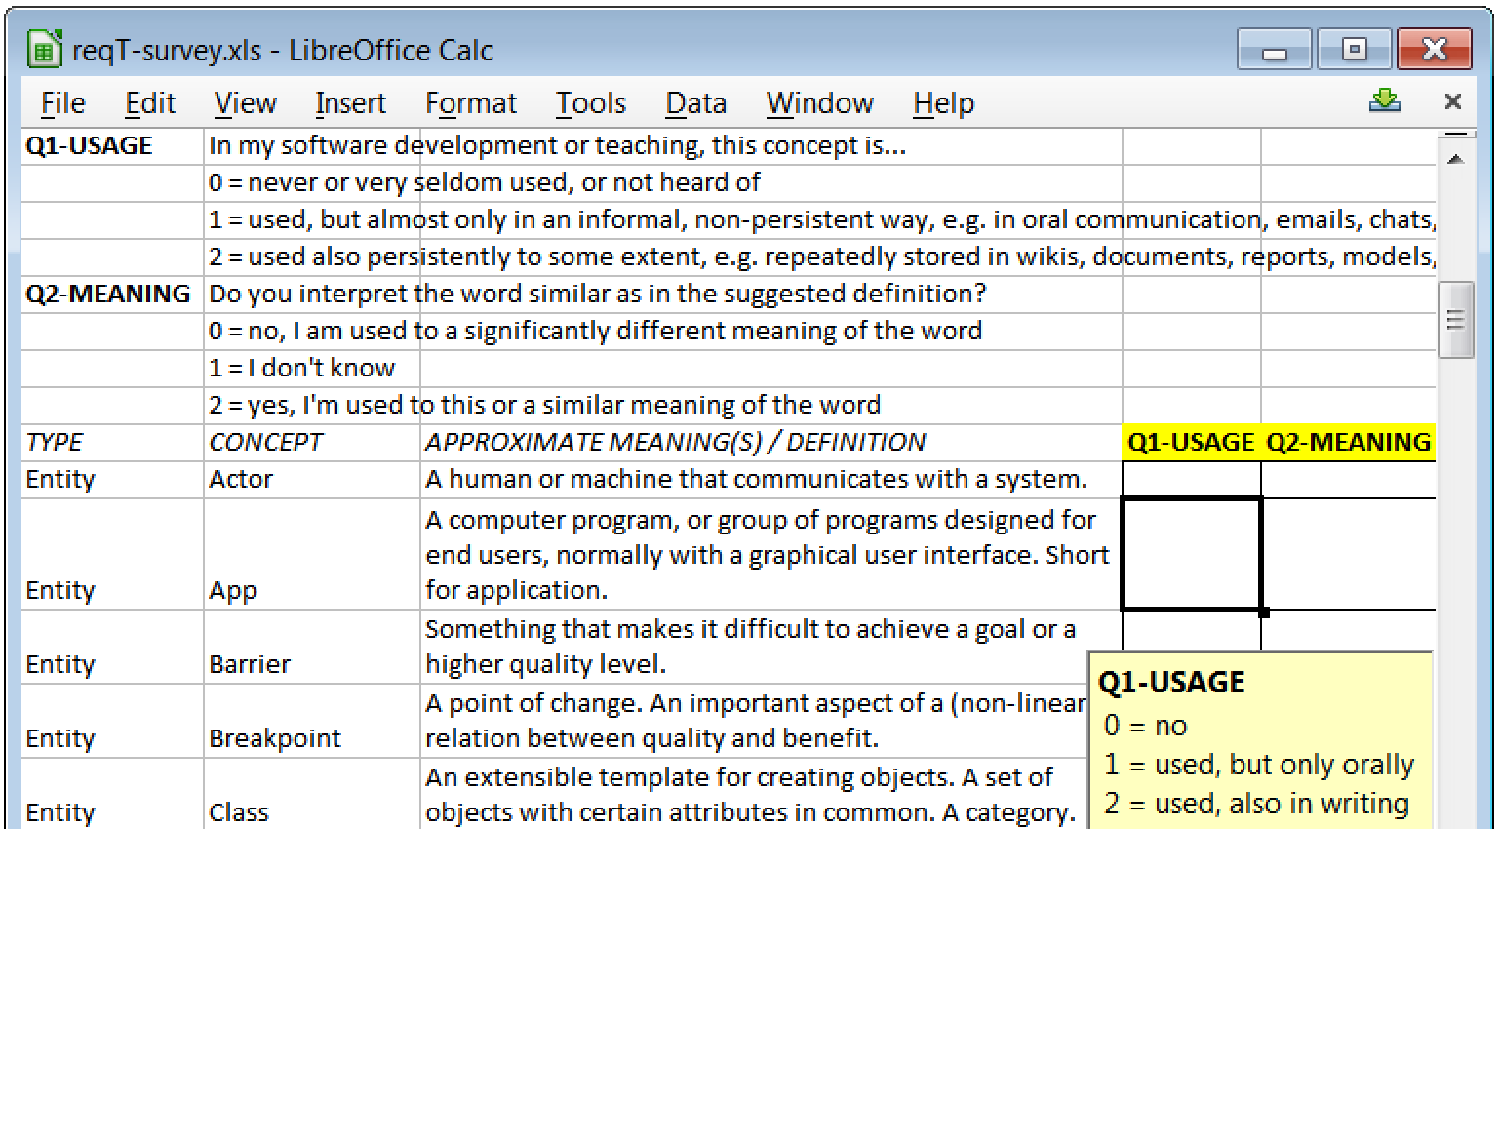
\includegraphics[width=0.75\textwidth]{img/survey-screen-dump}
\caption{Screen dump of survey instrument.}
\end{figure}
\section{Data Analysis}

\textbf{Subject background.} The background questions in the survey regards the role of the subject, as shown in Table \ref{table:background}. In summary, the included\footnote{One subject answered NO on all background questions and was therefore excluded.} %%% ====== Data Summary =======
total number of subjects is 14, 
of which 10 are teachers, 
10 are developers and 
13 are researchers.

\begin{table}[H]
\centering
\fontsize{8}{9}\selectfont
\caption{Background of subjects, $N = 15$. The table shows anonymized subject ids}
\label{table:background}
\begin{tabular}{p{0.42\textwidth}| p{0.58\textwidth}}
\textit{Question} & \textit{Subject responding YES}  \\ \hline
Do you teach software engineering and/or requirements engineering? YES/NO & S01 S03 S04 S05 S07 S08 S09 S11 S12 S14\\
Do you develop software by writing code and/or creating system models? YES/NO & S01 S02 S03 S07 S08 S09 S10 S11 S13 S14\\
Do you do academic research in software and/or requirements engineering? YES/NO & S01 S03 S04 S05 S06 S07 S08 S09 S10 S11 S12 S13 S14\\


 \end{tabular}
\end{table}

\textbf{Frequency analysis.} The idea of ''essentiality'' is characterized as the number of subjects that has responded that they (1) use the concepts at least in an informal, non-persistent way, and (2) use the concepts in a similar meaning as in the definition in Appendix A. Table \ref{table:frequency} shows the results of the frequency counts.  

%
\begingroup
\setlength{\tabcolsep}{4pt} % Default value: 6pt
\renewcommand{\arraystretch}{1.5} % Default value: 1
\begin{table}[H]
\centering
\fontsize{7}{8}\selectfont
\caption{Frequency analysis of concepts' ''essentiality'', where $n$ is the number of subjects that answered $(use >= 1)$ and $(agree = 2)$ for each concept.}
\label{table:frequency}
\begin{tabular}{l | p{0.33\textwidth} | p{0.30\textwidth} | p{0.25\textwidth}}
\textit{$n$} & \textit{Entities} & \textit{Attributes} & \textit{Relations} \\ \hline
%%%%%%%%%%%%% Summary table of (use, agree) >= (1, 2)
$14$ & \texttt{Class, Component, UseCase, Variant} & \texttt{Comment, Example, Max, Min, Title} & \texttt{implements, verifies}\\\hline
$13$ & \texttt{Configuration, Data, Design, Event, Quality, Scenario, Stakeholder, System, Term} & \texttt{Code, Constraints, Cost, FileName, Probability, Profit, Spec, Why} & \texttt{excludes, interactsWith, is, relatesTo, requires}\\\hline
$12$ & \texttt{Actor, Domain, Feature, Function, Interface, Module, Relationship, Release, Req, Risk, Service, State, Task, Test} & \texttt{Benefit, Capacity, Frequency, Input, Order, Output, Prio, Text, Value} & \texttt{has, impacts}\\\hline
$11$ & \texttt{Idea, Label, Member, Meta, MockUp, Section, User} & \texttt{Image} & \texttt{precedes, superOf}\\\hline
$10$ & \texttt{Goal, Story} & \texttt{Expectation} & \texttt{}\\\hline
$9$ & \texttt{App, Issue, Target, WorkPackage} & \texttt{Damage} & \texttt{binds, helps}\\\hline
$8$ & \texttt{Item, Product, Resource, VariationPoint} & \texttt{} & \texttt{deprecates}\\\hline
$7$ & \texttt{Breakpoint, Screen} & \texttt{Status} & \texttt{}\\\hline
$6$ & \texttt{Barrier} & \texttt{Deprecated} & \texttt{hurts}\\\hline
$5$ & \texttt{} & \texttt{} & \texttt{}\\\hline
$4$ & \texttt{Ticket} & \texttt{} & \texttt{}\\\hline
$3$ & \texttt{} & \texttt{} & \texttt{}\\\hline
$2$ & \texttt{} & \texttt{} & \texttt{}\\\hline
$1$ & \texttt{Epic} & \texttt{Gist} & \texttt{}\\\hline
$0$ & \texttt{} & \texttt{} & \texttt{}\\\hline

 \end{tabular}
\end{table}
\endgroup
%%%%%%%%%%%%%% DISCUSSION

\section{Discussion and Conclusion}\label{section:discussion}

!!Discuss and conclude!!



{\bf Limitations. } Due to the limited number of subjects and the high degree of homogeneity among subjects with respect to background, it is difficult to analyse and draw conclusions about potential differences in opinions between e.g. teachers and developers. Some subjects needed more time and completed survey offline during the coming days, which may give a variation in how careful the responses were considered. The survey was conducted by the author and inventor of reqT, in conjunction with a seminar and demo of reqT. In order to avoid any positive bias due to advocacy in favour of the reqT metamodel, the survey was held prior to the seminar and demo. This in turn may introduce a threat of limited knowledge among subjects of the idea behind the modelling approach in reqT 
 
{\bf Future work.} %Further directions of research include (1) incorporation of constraints on models for support of prioritization and release planning \cite{Regnell2011}, (2) more elaborate semantic checks to better guide requirements modelers, and (3) graphical visualization of requirements graph models. (4) Natural Language Processing technology including e.g. ambiguity risk detection may be interesting to combine with reqT. (5) It is also important to further investigate the pedagogic advantages and limitations of the approach. 

%A major objective of this research preview paper is to expose the latest version of reqT to the community of RE scholars and to invite discussions and contributions.


\subsubsection*{Acknowledgments.} This work is partly funded by  VINNOVA within the EASE project.

\bibliography{refs}
\bibliographystyle{splncs03}

%%%%%%%%%%%%%%% APPENDIX WITH DEFINITIONS
\clearpage
%\hspace{-0.9cm}
\section*{Appendix A: Definitions of Metamodel Concepts}
\begin{minipage}{1\linewidth}
\begin{minipage}{0.30\textwidth} 

\begin{table}[H]
%\centering
\vspace{-0.8cm}
\fontsize{6}{6.5}\selectfont
%\caption{.}%: Entities, Attributes and Relations.}

\begin{tabular}{|l p{4.5cm}|}
\hline
\textit{Entity} & \textit{Definition}  \\ \hline
\texttt{Actor}&A human or machine that communicates with a system.\\
\texttt{App}&A computer program, or group of programs designed for end users, normally with a graphical user interface. Short for application.\\
\texttt{Barrier}&Something that makes it difficult to achieve a goal or a higher quality level.\\
\texttt{Breakpoint}&A point of change. An important aspect of a (non-linear) relation between quality and benefit.\\
\texttt{Class}&An extensible template for creating objects. A set of objects with certain attributes in common. A category.\\
\texttt{Component}&A composable part of a system. A reusable, interchangeable system unit or functionality.\\
\texttt{Configuration}&A specific combination of variants.\\
\texttt{Data}&Information stored in a system.\\
\texttt{Design}&A specific realization or high-level implementation description (of a system part).\\
\texttt{Domain}&The application area of a product with its surrounding entities.\\
\texttt{Epic}&A large user story or a collection of stories.\\
\texttt{Event}&Something that can happen in the domain and/or in the system.\\
\texttt{Feature}&A releasable characteristic of a product. A (high-level, coherent) bundle of requirements.\\
\texttt{Function}&A description of how input data is mapped to output data. A capability of a system to do something specific.\\
\texttt{Goal}&An intention of a stakeholder or desired system property.\\
\texttt{Idea}&A concept or thought (potentially interesting).\\
\texttt{Interface}&A defined way to interact with a system.\\
\texttt{Issue}&Something needed to be fixed.\\
\texttt{Item}& An article in a collection, enumeration, or series.\\
\texttt{Label}&A descriptive name used to identify something.\\
\texttt{Member}&An entity that is part of another entity, eg. a field in a in a class.\\
\texttt{Meta}&A prefix used on a concept to mean beyond or about its own concept, e.g. metadata is data about data.\\
\texttt{MockUp}&A prototype with limited functionality used to demonstrate a design idea.\\
\texttt{Module}&A collection of coherent functions and interfaces.\\
\texttt{Product}&Something offered to a market.\\
\texttt{Quality}&A distinguishing characteristic or degree of goodness.\\
\texttt{Relationship}&A specific way that entities are connected.\\
\texttt{Release}&A specific version of a system offered at a specific time to end users.\\
\texttt{Req}&Something needed or wanted. An abstract term denoting any type of information relevant to the (specification of) intentions behind system development. Short for requirement.\\
\texttt{Resource}&A capability of, or support for development.\\
\texttt{Risk}&Something negative that may happen.\\
\texttt{Scenario}&A (vivid) description of a (possible future) system usage.\\
\texttt{Screen}&A design of (a part of) a user interface.\\
\texttt{Section}&A part of a (requirements) document.\\
\texttt{Service}&Actions performed by systems and/or humans to provide results to stakeholders.\\
\texttt{Stakeholder}&Someone with a stake in the system development or usage.\\
\texttt{State}&A mode or condition of something in the domain and/or in the system. A configuration of data.\\
\texttt{Story}&A short description of what a user does or needs. Short for user story.\\
\texttt{System}&A set of interacting software and/or hardware components.\\
\texttt{Target}&A desired quality level or goal .\\
\texttt{Task}&A piece of work (that users do, maybe supported by a system).\\
\texttt{Term}&A word or group of words having a particular meaning.\\
\texttt{Test}&A procedure to check if requirements are met.\\
\texttt{Ticket}&(Development) work awaiting to be completed.\\
\texttt{UseCase}&A list of steps defining interactions between actors and a system to achieve a goal.\\
\texttt{User}&A human interacting with a system.\\
\texttt{Variant}&An object or system property that can be chosen from a set of options.\\
\texttt{VariationPoint}&An opportunity of choice among variants.\\
\texttt{WorkPackage}&A collection of (development) work tasks.\\

\hline
 \end{tabular}
\end{table}
\end{minipage}
 \hspace{4em plus 1fill} 
\begin{minipage}{0.47\textwidth} 
 \begin{table}[H]
%\centering
\fontsize{6}{6.5}\selectfont
%\caption{Definitions of attributes and relations.}
\vspace{-0.8cm}
\label{table-entities}
\begin{tabular}{|l p{4.0cm}|}
 \hline
\textit{Attribute} & \textit{Definition}  \\ \hline
\texttt{Benefit}&A characterisation of a good or helpful result or effect (e.g. of a feature).\\
\texttt{Capacity}&The largest amount that can be held or contained (e.g. by a resource).\\
\texttt{Code}&A collection of (textual) computer instructions in some programming language, e.g. Scala. Short for source code.\\
\texttt{Comment}&A note that explains or discusses some entity.\\
\texttt{Constraints}&A collection of propositions that restrict the possible values of a set of variables.\\
\texttt{Cost}&The expenditure of something, such as time or effort, necessary for the implementation of an entity.\\
\texttt{Damage}&A characterisation of the negative consequences if some entity (e.g. a risk) occurs.\\
\texttt{Deprecated}&A description of why an entity should be avoided, often because it is superseded by another entity, as indicated by a 'deprecates' relation.\\
\texttt{Example}&A note that illustrates some entity by a  typical instance.\\
\texttt{Expectation}&The required output of a test in order to be counted as passed.\\
\texttt{FileName}&The name of a storage of serialized, persistent data.\\
\texttt{Frequency}&The rate of occurrence of some entity. \\
\texttt{Gist}&A short and simple description of an entity, e.g. a function or a test.\\
\texttt{Image}&(The name of) a picture of an entity.\\
\texttt{Input}&Data consumed by an entity, \\
\texttt{Max}&The maximum estimated or assigned (relative) value.\\
\texttt{Min}&The minimum estimated or assigned (relative) value.\\
\texttt{Order}&The ordinal number of an entity (1st, 2nd, ...).\\
\texttt{Output}&Data produced by an entity, e.g. a function or a test.\\
\texttt{Prio}&The level of importance of an entity. Short for priority.\\
\texttt{Probability}&The likelihood that something (e.g. a risk) occurs.\\
\texttt{Profit}&The gain or return of some entity, e.g. in monetary terms.\\
\texttt{Spec}&A (detailed) definition of an entity. Short for specification\\
\texttt{Status}&A level of refinement of an entity (e.g. a feature) in the development process. \\
\texttt{Text}&A sequence of words (in natural language).\\
\texttt{Title}&A general or descriptive heading.\\
\texttt{Value}&An amount. An estimate of worth.\\
\texttt{Why}&A description of intention. Rationale.\\


\hline
\textit{Relation} & \textit{Definition}  \\ \hline
\texttt{binds}&Ties a value to an option. A configuration binds a variation point.\\
\texttt{deprecates}&Makes outdated. An entity deprecates (supersedes) another entity.\\
\texttt{excludes}&Prevents a combination. An entity excludes another entity.\\
\texttt{has}&Expresses containment, substructure. An entity contains another entity.\\
\texttt{helps}&Positive influence. A goal helps to fulfil another goal.\\
\texttt{hurts}&Negative influence. A goal hinders another goal.\\
\texttt{impacts}&Some influence. A new feature impacts an existing component.\\
\texttt{implements}&Realisation of. A module implements a feature.\\
\texttt{interactsWith}&Communication. A user interacts with an interface.\\
\texttt{is}&Sub-typing, specialization, part of another, more general entity.\\
\texttt{precedes}&Temporal ordering. A feature precedes (is implemented before) another feature.\\
\texttt{relatesTo}&General relation. An entity is related to another entity.\\
\texttt{requires}&Requested combination. An entity is required (or wished) by another entity.\\
\texttt{superOf}&Super-typing, generalization, includes another, more specific entity.\\
\texttt{verifies}&Gives evidence of correctness. A test verifies the implementation of a feature.\\

 \hline
\end{tabular}
\end{table}

\end{minipage}
\end{minipage}


\end{document}
